\documentclass[xcolor=dvipsname]
{beamer}
\usetheme{Szeged}
\usepackage[utf8]{inputenc}
\usepackage{tikz}
\usetikzlibrary{arrows,shapes}
\usetikzlibrary{fadings}
\usetheme{Antibes}
\usecolortheme{beaver}
\usepackage{textpos}
\usepackage{graphicx}
\usepackage{mathtools}
\usepackage{amsmath}
\usepackage{booktabs}
\usepackage{appendixnumberbeamer}


\usepackage{algorithmic}
\usepackage{hyperref}
\mode<presentation>{}
%% preamble
\title{     Implementation of LDPC Decoder - Using AHIR Tool Chain} 
\author[Anurag Gupta]
{Anurag Gupta\\ Microelectronics (2015-17) \\
		\footnotesize  Instructor: Prof Madhav P. Desai}
\institute[IIT-Bombay] % (optional)
{
	\textit{IIT-Bombay\\
	Department of Electrical Engineering} \\ 
	
\includegraphics[height=1.5cm,width=1.5cm]{iitb_logo}
}
\newcommand\Fontbig{\fontsize{25}{7.2}\selectfont}
%\logo{
\includegraphics[height=1cm]{iitb_logo.jpg}}

%\usecolortheme{dolphin}

\addtobeamertemplate{navigation symbols}{}{%
	\usebeamerfont{footline}%
	\usebeamercolor[fg]{footline}%
	\hspace{1em}%
	\insertframenumber/\inserttotalframenumber
}
\setbeamercolor{footline}{fg=blue}



\setbeamertemplate{frametitle}[default]

%\usepackage{bbding}
\defbeamertemplate{itemize item}{boldarrow}{\ArrowBoldRightShort}

  \setbeamerfont{footnote}{size=\tiny}



\begin{document}


	%% title frame
	\begin{frame}[t]
		\titlepage
	\end{frame}
	
	\addtobeamertemplate{frametitle}{}{%
		\begin{textblock*}{100mm}(.90\textwidth,-1cm)
			
\includegraphics[height=1cm,width=1cm]{iitb_logo}
		\end{textblock*}}
%------------------------------------------------------------	
%%Table of content frame
\begin{frame}[t]
\frametitle{Outline}
\tableofcontents[hideallsubsections]
\end{frame}	
%-------------------------------------------------------------	

%-----------------------------------------------------------------	
\section{Motivation}		
		\begin{frame}
			\frametitle{ Motivation }
			\textit{Why LDPC ?}
			\begin{itemize}
			\setbeamertemplate{itemize item}[triangle]
			\item Channel capacity approaching codes\footnote[frame]{S.-Y. Chung, G. D. Forney, Jr., T. J. Richardson, and R. L. Urbanke, “On
the design of low-density parity-check codes within 0.0045 dB of the
Shannon limit,” IEEE Commun. Letters, vol. 5, no. 2, pp. 58–60, February
2001.}
			  \begin{itemize}
			  \item S.Y.Chung shannon limit approaching code: For a white Gaussian noise channel threshold within 0.0045 dB of the Shannon limit with block length of $10^7$.
			  \end{itemize}
			\item Decoding time varies linearly proportional to block length
			  \begin{itemize}
			  \item Parity check matrix is sparse
			  \end{itemize}
			  \item Decoder can be parallelized
				\begin{itemize}
			  \item Decoding algorithms are iterative
			  \end{itemize}
			\end{itemize}
		\end{frame}
%-----------------------------------------------------------------			
%------------------------------------------------------------------
\section{LDPC Decoding Algorithm}

%================================================

 \begin{frame}[t]
\frametitle{LDPC Decoding Algorithms}
\begin{itemize}
\item Hard decoding algorithms
	\begin{itemize}
	\item Bit flipping algorithm
	\end{itemize}
\item Soft decoding algorithms
	\begin{itemize}
	\item Sum product decoding
	\item Min sum decoding
	\end{itemize}
\end{itemize}
\end{frame}	

%===========================================

%=============================================================


\begin{frame}[t]
\frametitle{ Min Sum Decoding Algorithm }
\pause
\alert{Tanner Graph:}
	\begin{itemize}
	\item LDPC code's parity check equations can be represented by bipartite graph, called the Tanner graph\footnote{R. M. Tanner, “A recursive approach to low complexity codes,” IEEE
Trans. Inform. Theory, vol. IT-27, no. 5, pp. 533–547, September 1981.}.
	\end{itemize}

	\begin{columns}[totalwidth=\textwidth]
		\begin{column}{0.5\textwidth}
		\centering
\[
\begingroup % keep the change local
\setlength\arraycolsep{1pt}
\left[ \begin{array} {c|cccccccc} 
  &    c1 &   c2 &   c3 &  c4  &  c5  &  c6  &  c7  &  c8 \\ \hline
r1 &    1  &   1  &   1  &   0  &   0  &   0  &   0  &   0 \\
r2 &    0  &   0  &   0  &   1  &   1  &   1  &   0  &   0 \\ 
r3 &    1  &   0  &   0  &   1  &   0  &   0  &   1  &   0 \\
r4 &    0  &   1  &   0  &   0  &   1  &   0  &   0  &   1 \end{array} \right] 
\endgroup
\]			
	\end{column}%    		
	\begin{column}{0.5\textwidth}
		\centering
		\begin{figure}
		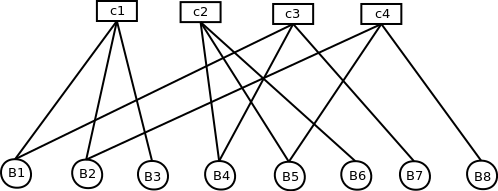
\includegraphics[height=3cm,width=6cm]{minSum1}
		\caption{ Tanner Graph }
	\end{figure}
	\end{column}%
\end{columns}
\end{frame}

%===================================================
\begin{frame}[t]
\frametitle{ A priori initialization }  
\begin{columns}[totalwidth=\textwidth]
	\begin{column}{0.4\textwidth}
	\centering
	\begin{itemize}
	\item A priories are calculated by soft information of the code bits.	
	\item 	$
	\alert{aPriori[I] =}
	$
	$
	\alert{ -4 * C[I] * R * \dfrac{Eb}{No}}
	$ 
	\item where C[I] = $i^{th}$ code block
	\item R = code rate
	\item $\dfrac{Eb}{No}$ = signal to noise power ratio
	\end{itemize}
 
			
	\end{column}% 
	   		
	\begin{column}{0.6\textwidth}
	\centering
	\begin{figure}
	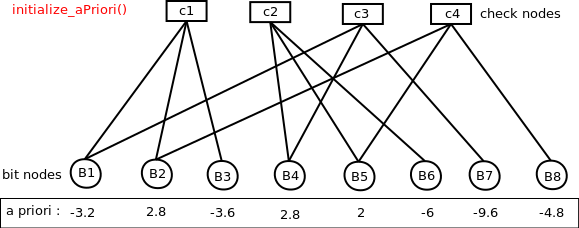
\includegraphics[height=4cm,width=7cm]{minSum2}
	\caption{ A priori initialization }
	\end{figure}
	\end{column}%
\end{columns}
\end{frame}


%======================================================

\begin{frame}[t]
\frametitle{ Message initialization }  
\begin{columns}[totalwidth=\textwidth]
	\begin{column}{0.4\textwidth}
	\centering
	\begin{itemize}
	\item Messages are the information propagating from bit nodes to check nodes.
	\item These are initialized to a priori of their respective bit node.	
	\item 	$ \alert{message[I][J] =} 
	$
	$
	\alert{aPriori[I]} 
	$ 
	\end{itemize}
 
			
	\end{column}% 
	   		
	\begin{column}{0.6\textwidth}
	\centering
	\begin{figure}
	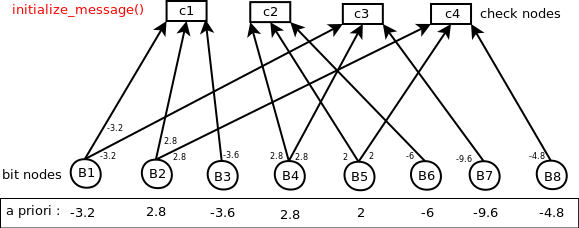
\includegraphics[height=4cm,width=7cm]{minSum3}
	\caption{ Message initialization }
	\end{figure}
	\end{column}%
\end{columns}
\end{frame}

%=======================================================

\begin{frame}[t]
\frametitle{ Extrinsic information calculation }  
\vspace{-5mm}
\begin{columns}[totalwidth=\textwidth]
	\begin{column}{0.3\textwidth}
	\centering
	\begin{itemize}
	\item Extrinsic information of a bit node is calculated as min sum of all the messages connected to 
	that particular check node. 	
	\end{itemize}
 
			
	\end{column}% 
	   		
	\begin{column}{0.7\textwidth}
	\centering
	\begin{figure}
	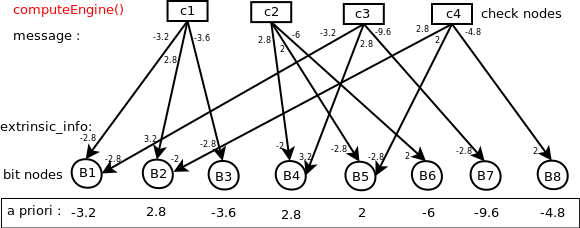
\includegraphics[height=4.5cm,width=8cm]{minSum4}
	\end{figure}
	\end{column}%
\end{columns}

\begin{itemize}

\item \alert{$|E_{(j,i)}| =  Min_{i'\in B_j \ i'\neq i }|M_{j,i'}|   $ }
\item \alert{$sign({E_{(j,i)}}) =  \prod_{i'\in B_j \ i'\neq i }sign(M_{j,i'})   $ }
\end{itemize}
\end{frame}

%======================================================
\begin{frame}[t]
\frametitle{ A posteriori calculation }  
\vspace{-5mm}
\begin{columns}[totalwidth=\textwidth]
	\begin{column}{0.3\textwidth}
	\centering
	\begin{itemize}
	\item A posteriori probabilities are the output bit probabilities.
	\item These are used to modify the code block after every iteration.
	\end{itemize}
 
			
	\end{column}% 
	   		
	\begin{column}{0.7\textwidth}
	\centering
	\begin{figure}
	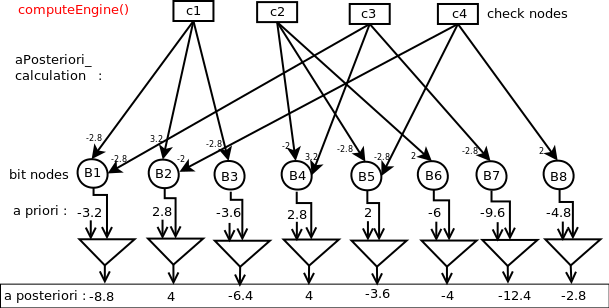
\includegraphics[height=4.5cm,width=8cm]{minSum5}
	\end{figure}
	\end{column}%
\end{columns}

\begin{itemize}

\item \alert{$ aPosteriori[I] = \sum_{j\in A_i} E_{j,i} + aPriori[I] $}
\end{itemize}
\end{frame}

%=====================================================
\begin{frame}[t]
\frametitle{ isDecoded block }  
\vspace{-5mm}
\begin{columns}[totalwidth=\textwidth]
	\begin{column}{0.48\textwidth}
	\centering
	\begin{itemize}
	\item This block flips a bit if it is different form hard decision 
	of the a posteriori probability of the bit. Thus, modifies the code block.  
	\item If, no bit got flipped then decoding stops.
	\end{itemize}
 
			
	\end{column}% 
	   		
	\begin{column}{0.52\textwidth}
	\centering
	\begin{figure}
	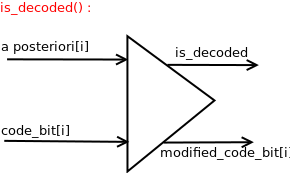
\includegraphics[height=3.5cm,width=5cm]{minSum6}
	\end{figure}
	\end{column}%
\end{columns}

\begin{itemize}

\item \alert{$ is\_decoded =  1$ ;\\
if $\forall$ i code\_bit[I] = hard\_decision(aPosteriori[I]) }
\end{itemize}
\end{frame}

%=====================================================
\begin{frame}[t]
\frametitle{ Updating messages }  
\vspace{-5mm}
\begin{columns}[totalwidth=\textwidth]
	\begin{column}{0.3\textwidth}
	\centering
	\begin{itemize}
	\item Messages are updated and transmitted back to start the next iteration of decoding.
	\end{itemize}
 
			
	\end{column}% 
	   		
	\begin{column}{0.7\textwidth}
	\centering
	\begin{figure}
	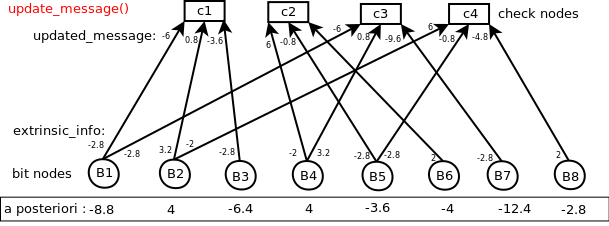
\includegraphics[height=5cm,width=8cm]{minSum7}
	\end{figure}
	\end{column}%
\end{columns}

\begin{itemize}

\item \alert{$   message_{(j,i)} = aPosteriori[i] - E_{(j,i)}  $}
\end{itemize}
\end{frame}

%-----------------------------------------------------------------------\subsection{Min Sum Decoding Algorithm}
 \begin{frame}[t]
 \alert{ LDPC Decoding : Min Sum Decode}
	\begin{figure}[h]
    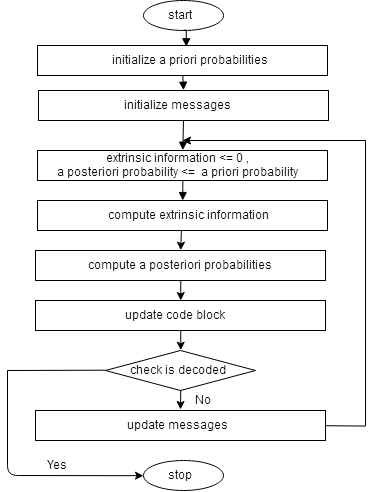
\includegraphics[height=6.5cm,width=5cm]{minSumDecode_flowChart}
    \end{figure}
\end{frame}	

%=======================================================	
\section{Decoder Implementation}
				\begin{frame} 
					\frametitle{ Decoder Implementation }
  Three different implementation\footnote{Muhammad Awais and Carlo Condo, "Flexible LDPC Decoder Architectures," VLSI Design, vol. 2012, Article ID 730835, 16 pages, 2012.} strategies are possible.
						\begin{enumerate}
							\item Serial decoder
							\begin{itemize}
							\item simple
							\item cheap
							\item slow
							\end{itemize}
							\item Fully parallel decoder
							\begin{itemize}
							\item complex
							\item costly
							\item Super fast
							\end{itemize}
							\item Partial parallel decoder. \\
\textit{"Can we effectively partition a bipartite graph corresponding to a LDPC parity check matrix ?"	}					
						\end{enumerate}
				\end{frame}	

%========================================================

\subsection{Implementation of Serial Decoder }

%=====================================================

\begin{frame}[t]
\frametitle{ Implementation of Serial Decoder }  

\end{frame}

\begin{frame}[t]
\begin{figure}
       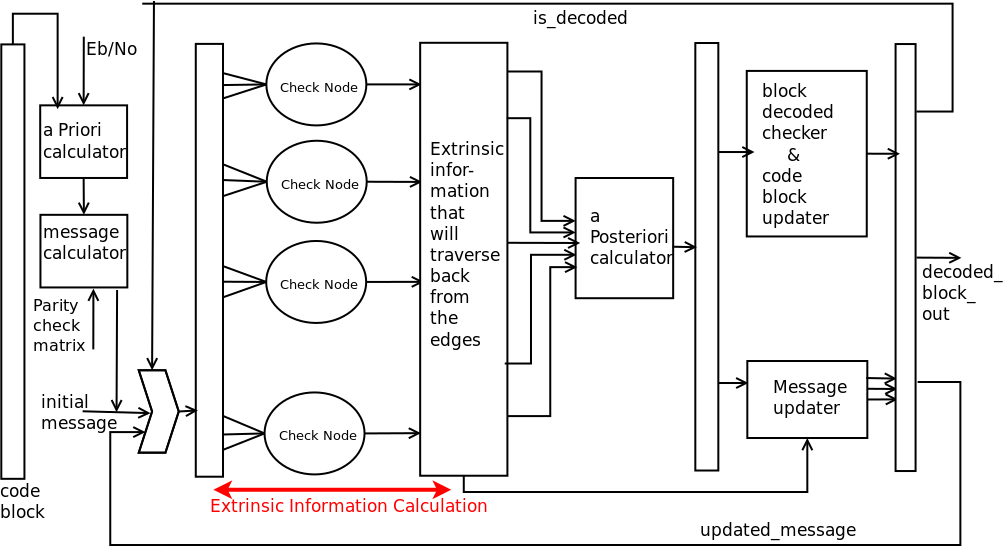
\includegraphics[height=6.5cm,width=11cm]{minSum}
       \end{figure}
\end{frame}
%=======================================================
\subsubsection{C Level Implementation \& Testing}


\begin{frame}[t]
\frametitle{C Level Implementation \& Testing }

\end{frame}
%===================================================
\begin{frame}[t]
\frametitle{ Serial Min Sum Decoder - Quasi-Cyclic Matrix }
\begin{itemize}
\item Min sum algorithm is implemented for Gaussian channel. 
\item Quasi-cyclic matrix of block size(n=) 4K, 8K and 12K  are formed using Sridhara-Fuja-Tanner algorithm.
\item Five different code rates(R=) 0.75, 0.80, 0.85, 0.90 and 0.95 are taken.
\item Raw input bit error rate(BER(IN)) is between $10^{-2}$ to $10^{-3}$, converted in form of Eb/No(db) to express input SNR in db. 
\item BER(OUT) : Output block error rate.
\item We have tabulated when the first code block get wrongly decoded till 1 million transmitted blocks.
\end{itemize}
\end{frame}
	
\begin{frame}[t] 
\frametitle{First error till 1 million blocks}

\begin{table}[]
\centering
\begin{tabular}{|l|l|r|r|}
\hline
n$\simeq$   & BER(In)$\simeq$    & R=0.75  & R=0.80  \\ \hline
4K  & $1.0x10^{-2}$  & -    & -       \\ 
    & $0.5x10^{-3}$  &-     & -       \\ 
    & $1.0x10^{-3}$  & -   & -       \\ \hline
8K  & $1.0x10^{-2}$   & -   & -           \\
    & $0.5x10^{-3}$ & -     & -       \\ 
    & $1.0x10^{-3}$   & -   & -                 \\ \hline
12K & $1.0x10^{-2}$   & -   & -        \\ 
    & $0.5x10^{-3}$ & -     & -     \\
    & $1.0x10^{-3}$   & - & -		\\ \hline 
\end{tabular}
\end{table}
\begin{itemize}
\item -	 : No error found till 1 million blocks. 
\end{itemize}
\end{frame}


\begin{frame}[t] 
\frametitle{First error till 1 million blocks}

\begin{table}[]
\centering
\begin{tabular}{|l|l|r|r|r|}
\hline
n$\simeq$   & BER(In)$\simeq$  & R=0.85  & R=0.9 & R=0.95 \\ \hline
4K  & $1.0x10^{-2}$    &2.677$x10^{3}$           &1.7819$x10^{4}$       &1       \\ 
    & $0.5x10^{-3}$    &2.4944$x10^{4}$          &1.65511$x10^{5}$		&1.79$x10^{2}$   \\ 
    & $1.0x10^{-3}$    &5.47550$x10^{5}$         &4.89654$x10^{5}$     &3.328$x10^{3}$ \\ \hline
8K  & $1.0x10^{-2}$    &2.3817$x10^{4}$          &1.16847$x10^{5}$        &1   \\ 
    & $0.5x10^{-3}$    &6.9491$x10^{4}$          &1.72263$x10^{5}$        &1.001$x10^{3}$  \\ 
    & $1.0x10^{-3}$    &9.16505 $x10^{5}$        &6.28939$x10^{5}$       &9.338$x10^{3}$           \\ \hline
12K & $1.0x10^{-2}$    &9.705$x10^{3}$          &5.37754$x10^{5}$       	&1       \\
    & $0.5x10^{-3}$    &5.6400$x10^{4}$          &-     			 		&1.318$x10^{3}$             \\ 
    & $1.0x10^{-3}$    &- 			             &-    					 &1.6920$x10^{4}$   \\ \hline 
\end{tabular}
\end{table}
\begin{itemize}
\item -	 : No error found till 1 million blocks. 
\end{itemize}
\end{frame}

\begin{frame}[t]
\frametitle{ Serial Min Sum Decoder - Random Matrix }

\begin{itemize}
\item Min sum algorithm is implemented for Gaussian channel. 
\item Random matrix of block size(n=) 4K, 8K and 12K  are formed using Mackey's algorithm.
\item Five different code rates(R=) 0.75, 0.80, 0.85, 0.90 and 0.95 are taken.
\item Raw input bit error rate(BER(IN)) is between $10^{-2}$ to $10^{-3}$, converted in form of Eb/No(db) to express input SNR in db. 
\item BER(OUT) : Output bit error rate.
\item We have tabulated when the first block get wrongly decoded till 1 million transmitted blocks.
\end{itemize}
\end{frame}	


\begin{frame}[t] 
\frametitle{First error in 1 million blocks}

\begin{table}[]
\centering
\begin{tabular}{|l|l|r|r|}
\hline
n$\simeq$   & BER(In)$\simeq$    & R=0.75  & R=0.8  \\ \hline
4K  & $1.0x10^{-2}$  &  1.2799$x10^{4}$    & 2.0754$x10^{4}$           \\ 
    & $0.5x10^{-3}$  &  5.53727$x10^{5}$    &  1.72781$x10^{5}$       \\ 
    & $1.0x10^{-3}$   & -				   & 6.24436$x10^{5}$       \\ \hline
8K  & $1.0x10^{-2}$   & 1.92476$x10^{5}$   & 8.3898$x10^{4}$        \\ 
    & $0.5x10^{-3}$   & 3.21027$x10^{5}$     & 4.6092$x10^{4}$        \\ 
    & $1.0x10^{-3}$   & -				   & -                 \\ \hline
12K & $1.0x10^{-2}$   & 2.20022$x10^{5}$   & 1.57371$x10^{5}$          \\ 
    & $0.5x10^{-3}$   & 2.17452$x10^{5}$     & 9.0158$x10^{4}$        \\ 
    & $1.0x10^{-3}$   & -				     & -        \\ \hline   
\end{tabular}
\end{table}
\begin{itemize}
\item -	 : No error found till 1 million blocks. 
\end{itemize}
\end{frame}

\begin{frame}[t] 
\frametitle{First error in 1 million blocks}

\begin{table}[]
\centering
\begin{tabular}{|l|l|r|r|r|}
\hline
n$\simeq$   & BER(In)$\simeq$    & R=0.85  & R=0.9 & R=0.95 \\ \hline
4K  & $1.0x10^{-2}$        & 3.39$x10^{2}$           & 1.259$x10^{3}$        & NA      \\ 
    & $0.5x10^{-3}$        & 6.6700$x10^{4}$        & 1.65511$x10^{5}$               & NA   \\ 
    & $1.0x10^{-3}$        & 3.45503$x10^{5}$        & 1.19008$x10^{5}$        & NA  \\ \hline
8K  & $1.0x10^{-2}$        & 5.193$x10^{3}$         & 5.947$x10^{3}$         & NA      \\ 
    & $0.5x10^{-3}$        & 3.7952$x10^{4}$        & 1.1389$x10^{4}$          & NA  \\ 
    & $1.0x10^{-3}$        & -             			& -               		 & NA             \\ \hline
12K & $1.0x10^{-2}$        & 1.2894$x10^{4}$        & 1.2626$x10^{4}$     & 1.1      \\ 
    & $0.5x10^{-3}$        & 1.56487$x10^{5}$      & 5.4866$x10^{4}$     & 1.034$x10^{4}$    \\ 
    & $1.0x10^{-3}$        & -			  			 & -           		& 1.4759$x10^{4}$   \\ \hline
      
\end{tabular}
\begin{itemize}
\item NA : Not Applicable. (Matrix was not formed)
\item -	 : No error found till 1 million blocks. 
\end{itemize}
\end{table}
\end{frame}		

\subsubsection{Aa to VHDL}
%====================================================
\begin{frame}[t]
\frametitle{Aa to VHDL -AHIR Tool Chain\footnote{https://github.com/madhavPdesai/ahir/release/docs/pdf/Overview.pdf.} }  
\pause
\begin{figure}
       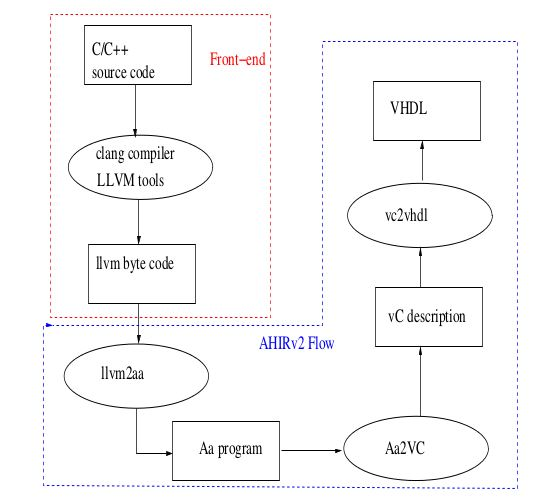
\includegraphics[height=5cm,width=8cm]{aa2vhdl}
       \end{figure}
\end{frame}
%======================================================
\begin{frame}[t]
\frametitle{Results} 
\vspace{-0.5cm} 
\begin{figure}
       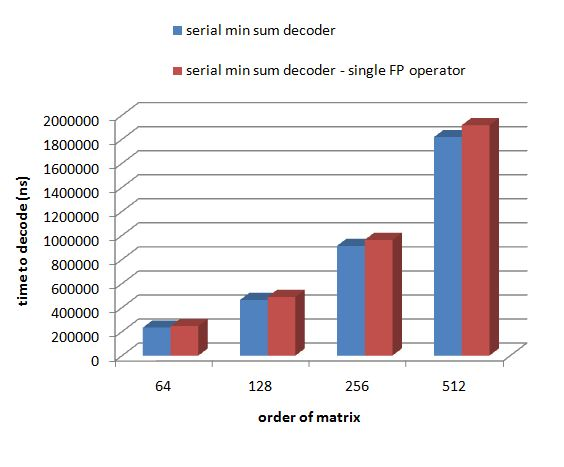
\includegraphics[height=7cm,width=10cm]{serialresult1}
       \end{figure}
\end{frame}
%=====================================================
\begin{frame}[t]
\frametitle{Results}  
\vspace{-0.5cm}
\begin{figure}

       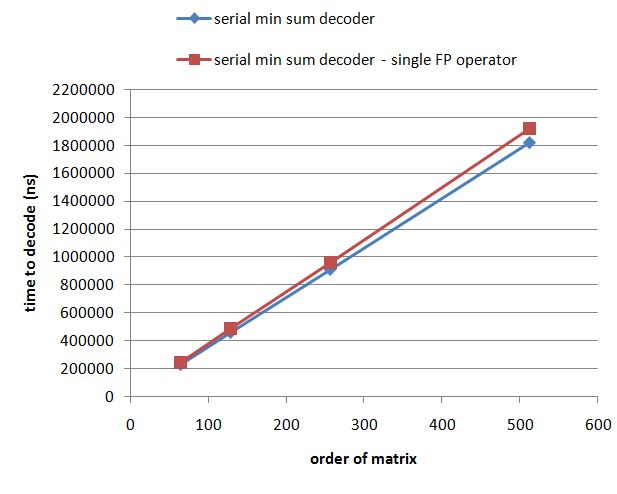
\includegraphics[height=7cm,width=10cm]{serialresult2}
       \end{figure}
\end{frame}

%=====================================================
\begin{frame}[t]
\frametitle{Results : Hardware generated after \\ synthesising the design}
\begin{table}[]
\centering
\begin{tabular}{|p{1.3cm}|p{3.5cm}|p{3.5cm}|}
\hline
	& serial min sum decoder & serial min sum decoder \newline
	(single FP unit)  \\ \hline
FF & 18,076		&19,034		 \\ \hline
LUT & 19,502  &20,621  \\ \hline
Memory LUT & 6 & 3  \\ \hline 
I/O & 128 & 128  \\ \hline
BRAM & 56 & 56  \\ \hline
BUFG  & 1 & 1  \\ \hline
\end{tabular}
\end{table}
\end{frame}
%======================================================											

									
\subsubsection{Partitioning }
\begin{frame}[t] 
		\frametitle{ Partitioning : Objective }
		\begin{figure}
		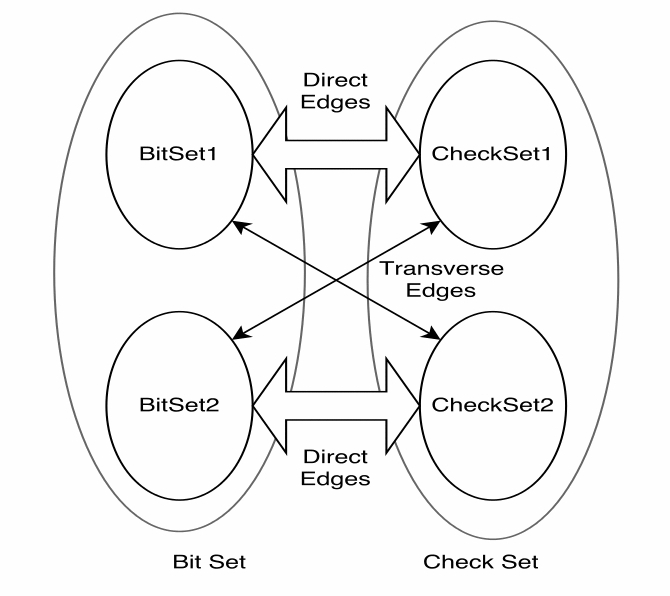
\includegraphics[height=5.5cm,width=5.5cm]{partition}
				\caption{Partitioning the bipartite graph}
			\end{figure}
	\end{frame}		
	
%----------------------------------------------------------------		

	
\subsubsection{Suggested Approach}
			\begin{frame}[t] 
		\frametitle{ Suggested Approach }
	
		\begin{figure}
		\hspace{-10mm}
		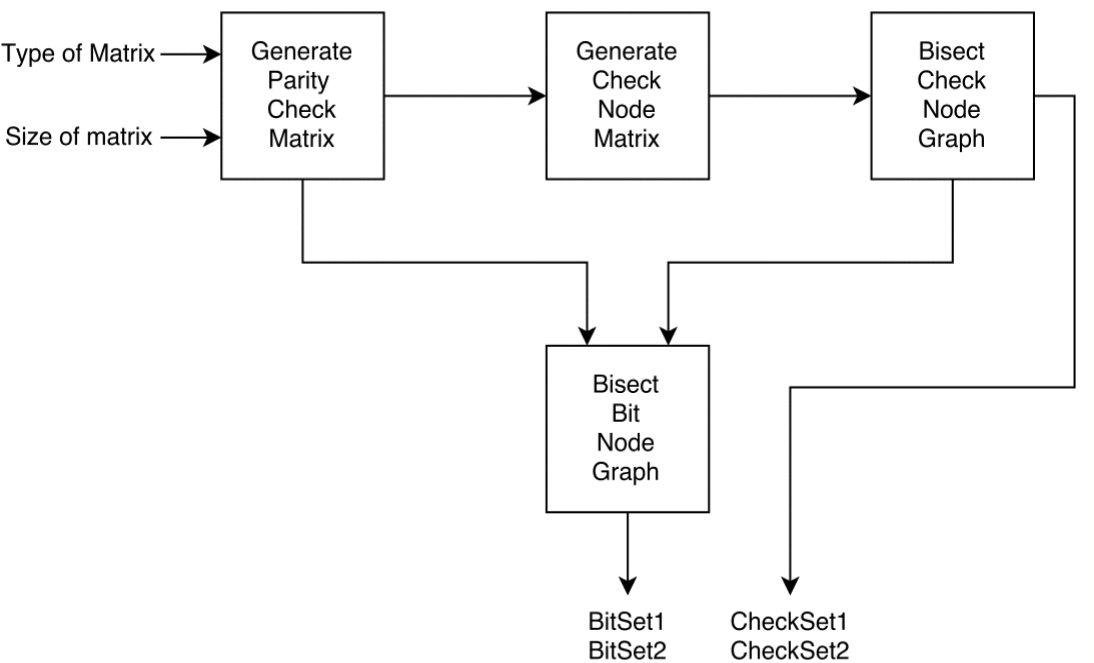
\includegraphics[height=5.5cm,width=9cm]{block.jpg}
				\caption{ Block diagram }
			\end{figure}
		
	\end{frame}	


\subsubsection{Partitioning Bit Node Set }

		\begin{frame}[t] 
\frametitle{ Partitioning Bit Node Set  }
\begin{columns}
\column{.5\textwidth}
\begin{figure}
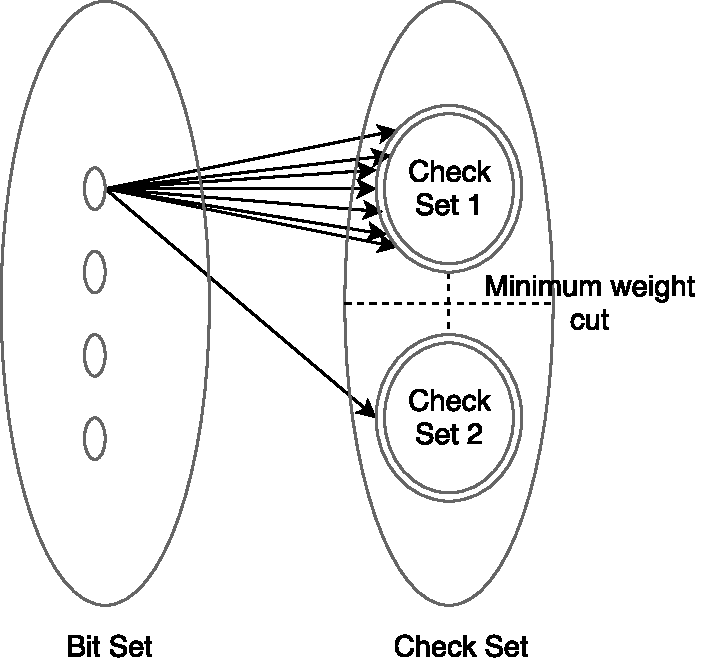
\includegraphics[height=5cm,width=5cm]{bitnodepar}
\caption{ After partitioning check node set }
			\end{figure}

\column{.5\textwidth}
\begin{figure}
				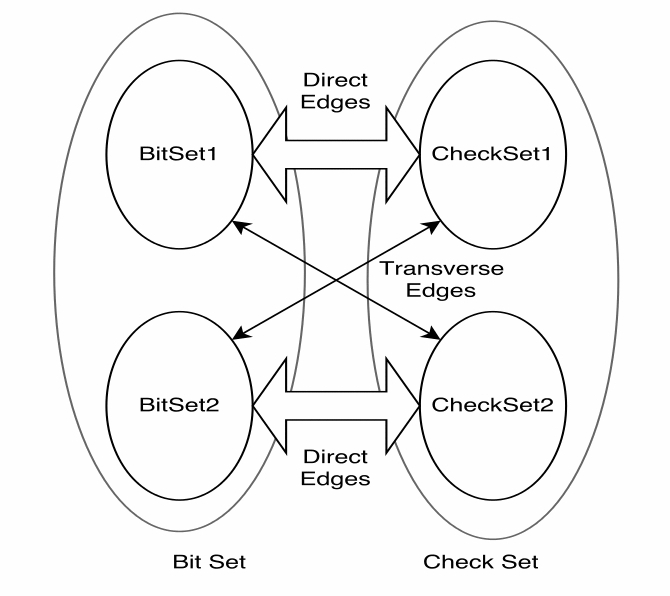
\includegraphics[height=5cm,width=5cm]{partition}
				\caption{ After partitioning bit node set}
			\end{figure}
\end{columns}
		\end{frame}		
%--------------------------------------------------------				
\subsubsection{Results }	
		\subsubsection{Gallager Parity Check Matrix}	
		\begin{frame}[t] 
			\frametitle{Gallager Parity Check Matrix}
			
			\begin{figure}
				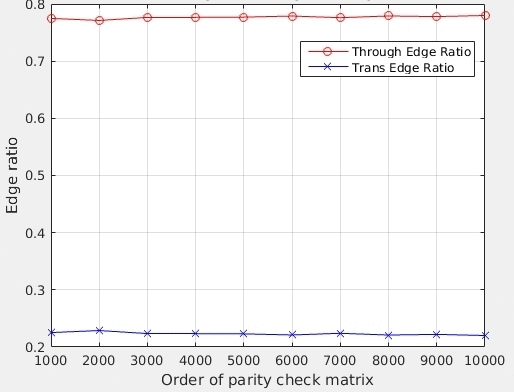
\includegraphics[height=6cm,width=8cm]{gallager}
			\end{figure}
			
		\end{frame}
		
		\subsubsection{Mackay Neal Parity Check Matrix}
		\begin{frame}[t] 
			\frametitle{Mackay Parity Check Matrix}
			
			\begin{figure}
				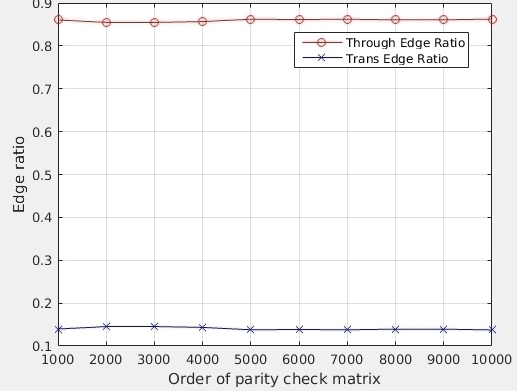
\includegraphics[height=6cm,width=8cm]{mackey}
			\end{figure}
		\end{frame}
		
		\subsubsection{Quasi Cyclic Parity Check Matrix}
		\begin{frame}[t] 
			\frametitle{Quasi Cyclic Parity Check Matrix}
			\begin{figure}
				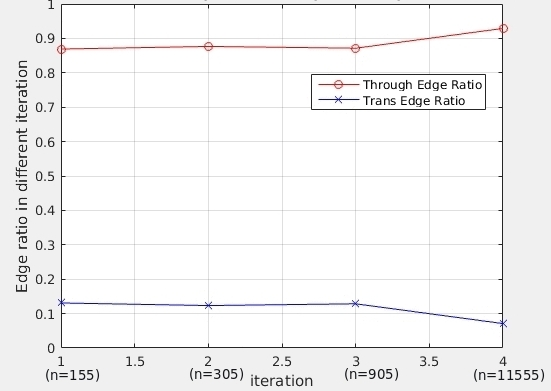
\includegraphics[height=6cm,width=8cm]{QC}
			\end{figure}
		\end{frame}


%-------------------------------------------------------------------
\subsection{Modified min sum algorithm}
\begin{frame}[t]
\pause
\frametitle{Modifying min sum algorithm using partitioning }  
\begin{itemize}
\item After partitioning the matrix we get four matrices as follows 	:
\[
H = \left[ \begin{array}{c|c}  
H11  & H12     \\ \hline
H21  & H22     \end{array} \right] 
\] 
\item example :
\[
\begingroup % keep the change local
\setlength\arraycolsep{1pt}
\left[ \begin{array} {c|cccccccc} 
  &    c1 &   c2 &   c3 &  c4  &  c5  &  c6  &  c7  &  c8 \\ \hline
r1 &    1  &   1  &   1  &   0  &   0  &   0  &   0  &   0 \\
r2 &    0  &   0  &   0  &   1  &   1  &   1  &   0  &   0 \\ 
r3 &    1  &   0  &   0  &   1  &   0  &   0  &   1  &   0 \\
r4 &    0  &   1  &   0  &   0  &   1  &   0  &   0  &   1 \end{array} \right] 
     \Rightarrow
\left[ \begin{array} {c|cccc|cccc} 
  &    c4 &   c6 &   c7 &  c1  &  c2  &  c3  &  c8  &  c5 \\ \hline  
r2 &     1  &   1  &   0  &   0  &   0  &   0  &   0  &   1 \\
r3 &     1  &   0  &   1  &   1  &   0  &   0  &   0  &   0 \\ \hline
r1 &     0  &   0  &   0  &   1  &   1  &   1  &   0  &   0 \\
r4 &     0  &   0  &   0  &   0  &   1  &   0  &   1  &   1 \end{array} \right] 
\endgroup
\]
\item H12 and H21 are highly sparse.
\end{itemize}
\end{frame}







\begin{frame}[t]
\frametitle{ A priori initialization }  
\begin{columns}[totalwidth=\textwidth]
	\begin{column}{0.4\textwidth}
	\centering
	\begin{itemize}
	\item A priories are calculated by soft information of the code bits.	
	\item 	$
	\alert{aPriori[I] =}
	$
	$
	\alert{ -4 * C[I] * R * \dfrac{Eb}{No}}
	$ 
	\item where C[I] = $i^{th}$ code block
	\item R = code rate
	\item $\dfrac{Eb}{No}$ = signal to noise power ratio
	\end{itemize}
 
			
	\end{column}% 
	   		
	\begin{column}{0.6\textwidth}
	\centering
	\begin{figure}
	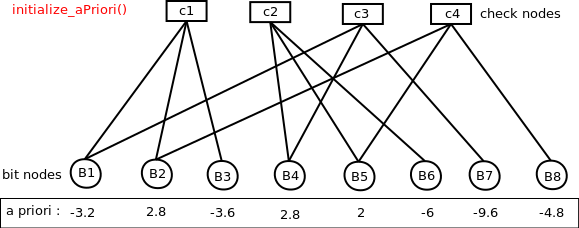
\includegraphics[height=4cm,width=7cm]{minSum2}
	\caption{ A priori initialization }
	\end{figure}
	\end{column}%
\end{columns}
\end{frame}


\begin{frame}[t]
\frametitle{ A priori initialization }  
\vspace{-5mm}
\begin{figure}
       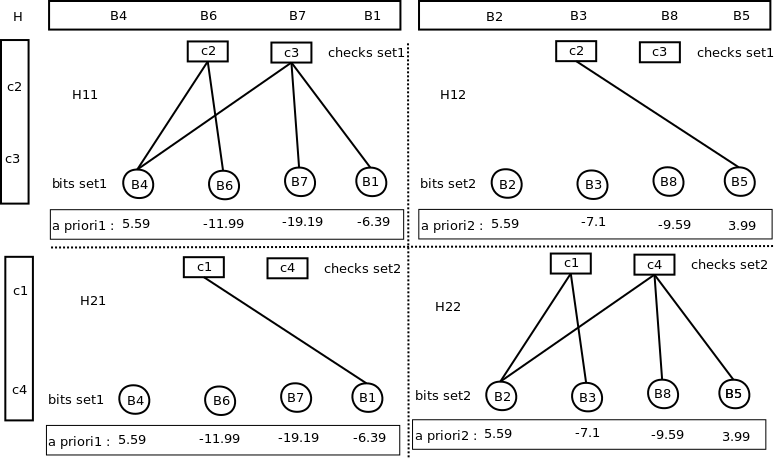
\includegraphics[height=6.5cm,width=11cm]{minSumModified1}
       \end{figure}
\end{frame}


\begin{frame}[t]
\frametitle{ Message initialization }  
\begin{columns}[totalwidth=\textwidth]
	\begin{column}{0.4\textwidth}
	\centering
	\begin{itemize}
	\item Messages are the information propagating from bit nodes to check nodes.
	\item These are initialized to a priori of their respective bit node.	
	\item 	$ \alert{message[I][J] =} 
	$
	$
	\alert{aPriori[I]} 
	$ 
	\end{itemize}
 
			
	\end{column}% 
	   		
	\begin{column}{0.6\textwidth}
	\centering
	\begin{figure}
	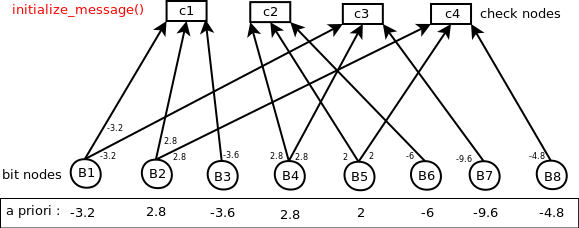
\includegraphics[height=4cm,width=7cm]{minSum3}
	\caption{ Message initialization }
	\end{figure}
	\end{column}%
\end{columns}
\end{frame}


\begin{frame}[t]
\frametitle{ Message initialization }  
\vspace{-5mm}
\begin{figure}
       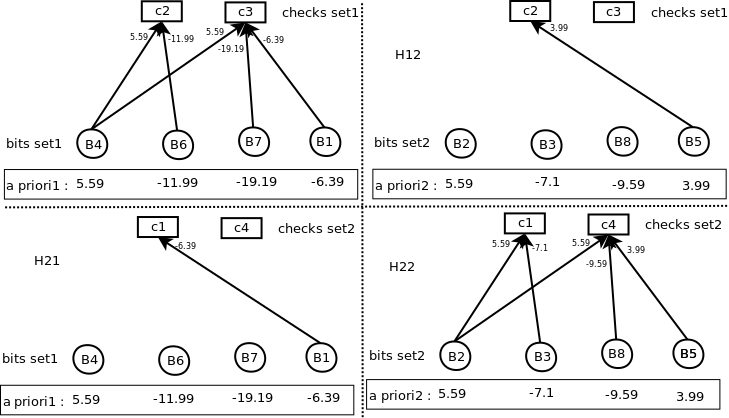
\includegraphics[height=6.5cm,width=11cm]{minSumModified2}
       \end{figure}
\end{frame}


\begin{frame}[t]
\frametitle{ Extrinsic information calculation }  
\vspace{-5mm}
\begin{columns}[totalwidth=\textwidth]
	\begin{column}{0.3\textwidth}
	\centering
	\begin{itemize}
	\item Extrinsic information of a bit node is calculated as min sum of all the messages connected to 
	that particular check node. 	
	\end{itemize}
 
			
	\end{column}% 
	   		
	\begin{column}{0.7\textwidth}
	\centering
	\begin{figure}
	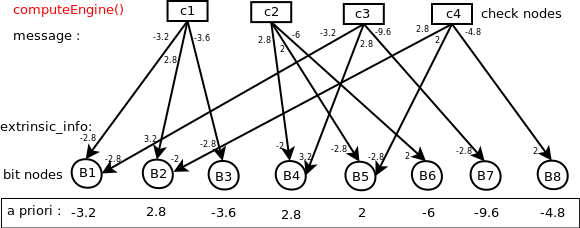
\includegraphics[height=4.5cm,width=8cm]{minSum4}
	\end{figure}
	\end{column}%
\end{columns}

\begin{itemize}

\item \alert{$|E_{(j,i)}| =  Min_{i'\in B_j \ i'\neq i }|M_{j,i'}|   $ }
\item \alert{$sign({E_{(j,i)}}) =  \prod_{i'\in B_j \ i'\neq i }sign(M_{j,i'})   $ }
\end{itemize}
\end{frame}

\begin{frame}[t]
\frametitle{ Partial Extrinsic information calculation }  
\vspace{-5mm}
\begin{figure}
       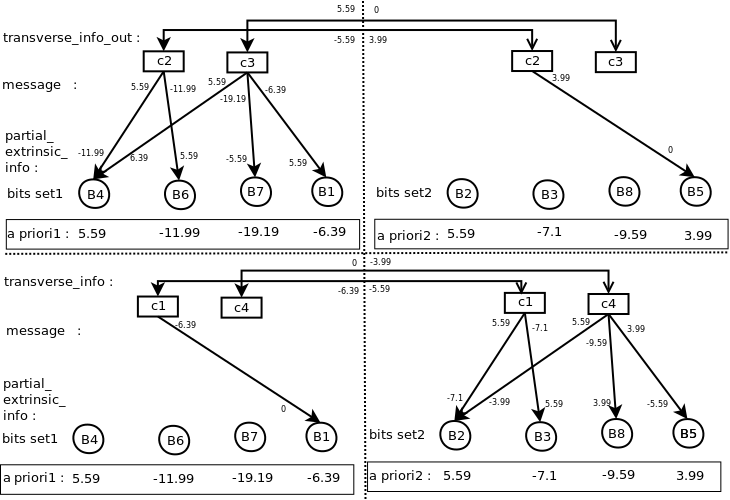
\includegraphics[height=6.5cm,width=11cm]{minSumModified3}
       \end{figure}
\end{frame}

\begin{frame}[t]
\frametitle{ Update extrinsic information }  
\vspace{-5mm}
\begin{figure}
       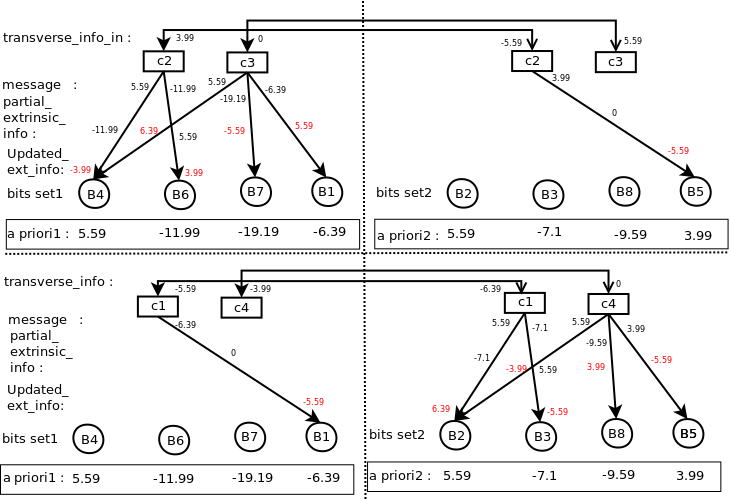
\includegraphics[height=6.5cm,width=11cm]{minSumModified4}
       \end{figure}
\end{frame}

%====================================================

\subsubsection{C Level Implementation}
%======================================================


\begin{frame}[t]
\frametitle{C Level Implementation}  

\end{frame}

\begin{frame}[t]
\frametitle{  }  
\begin{figure}
       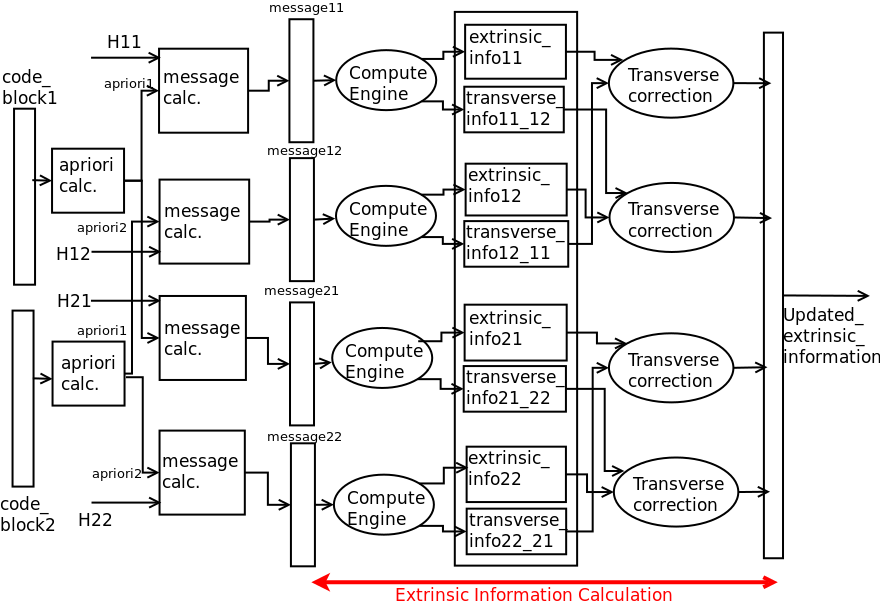
\includegraphics[height=7cm,width=11cm]{minSumModified}
       \end{figure}
\end{frame}

\begin{frame}[t]
\frametitle{  }                                 % and a label for
\alert{ modifiedMinSumDecode()	: }
\begin{algorithmic}                   
    \STATE $initialize\_aPriori(aPriori1) $
    \STATE $initialize\_aPriori(aPriori2) $
    \STATE $initializeMessage(message11) $
    \STATE $initializeMessage(message12) $
    \STATE $initializeMessage(message21) $
    \STATE $initializeMessage(message22) $
    \WHILE{$nitr \geq Max\_nitr$}    
    	\STATE$ initialize\_aPosteriori(aPosteriori1) \Leftarrow aPriori1 $
    	\STATE$ initialize\_aPosteriori(aPosteriori2) \Leftarrow aPriori2 $
   		\STATE $initializeExtrinsicInfo(ext\_info11) \Leftarrow 0 $
   		\STATE $initializeExtrinsicInfo(ext\_info12) \Leftarrow 0 $
   		\STATE $initializeExtrinsicInfo(ext\_info21) \Leftarrow 0 $
   		\STATE $initializeExtrinsicInfo(ext\_info22) \Leftarrow 0 $
   		\STATE ... 
   		\vspace{2cm}		
   		 \ENDWHILE 
\end{algorithmic}
\end{frame}


%========================================================
\begin{frame}[t]
\frametitle{  }                                 % and a label for
\alert{ modifiedMinSumDecode()	: }
\begin{algorithmic}   
\WHILE{...} 
\STATE ...               
\STATE$computeEngine(H11,message11,ext\_info11,trans\_info11\_12)$
\STATE$computeEngine(H22,message22,ext\_info22,trans\_info22\_12)$
\STATE$computeEngine(H12,message12,ext\_info12,trans\_info12\_11)$
\STATE$computeEngine(H21,message21,ext\_info21,trans\_info21\_22)$
\STATE$transverseCorrection(H11,transverse\_info12\_11,ext\_info11)$
\STATE$transverseCorrection(H22,transverse\_info21\_22,ext\_info22)$
\STATE$transverseCorrection(H21,transverse\_info22\_21,ext\_info21)$
\STATE$transverseCorrection(H12,transverse\_info11\_12,ext\_info12)$
\STATE$update\_aPosteriori (H11 , ext\_info11 ,aPosteriori1)$
\STATE$update\_aPosteriori (H22 , ext\_info22 ,aPosteriori2)$
\STATE$update\_aPosteriori (H12 , ext\_info12 ,aPosteriori1)$
\STATE$update\_aPosteriori (H21 , ext\_info21 ,aPosteriori2)$
\STATE ... \\
     ....	
 \ENDWHILE    


  		
\end{algorithmic}
\end{frame}


\begin{frame}[t]
\frametitle{  }                                 % and a label for
\alert{ modifiedMinSumDecode()	: }
\begin{algorithmic}   
\WHILE{...} 
\STATE ...  
\STATE$is\_decoded1 = checkIsdecoded( code\_block1 , aPosteriori1 ) $
\STATE$is\_decoded2 = checkIsdecoded( code\_block2 , aPosteriori2 ) $              
		\IF{$(is\_decoded1 \&\& is\_decoded2)== 1$}
        	\STATE break 
    	\ELSE
        	\STATE $updateMessage(ext\_info11 ,aPosteriori1 ,message11)$
        	\STATE $updateMessage(ext\_info22 ,aPosteriori2 ,message22)$
        	\STATE $updateMessage(ext\_info12 ,aPosteriori1 ,message12)$
        	\STATE $updateMessage(ext\_info21 ,aPosteriori2 ,message21)$
     	\ENDIF 
\STATE $nitr++$  
 \ENDWHILE     		
\end{algorithmic}
\end{frame}


%---------------------------------------------------------------
\subsubsection{Aa to VHDL}
%====================================================
\begin{frame}[t]
\frametitle{Aa to VHDL -AHIR Tool Chain\footnote{https://github.com/madhavPdesai/ahir/release/docs/pdf/Overview.pdf.} }  
\pause
\begin{figure}
       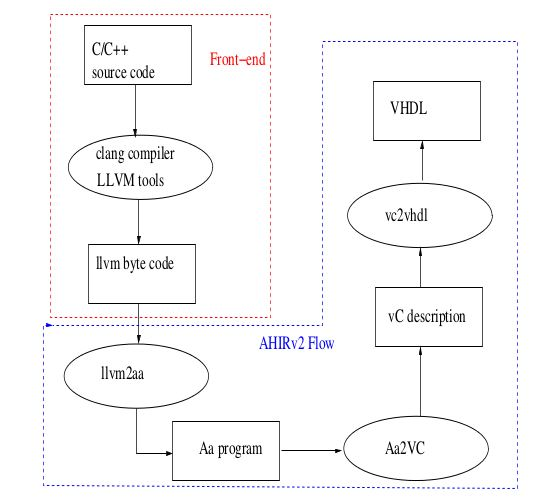
\includegraphics[height=5cm,width=8cm]{aa2vhdl}
       \end{figure}
\end{frame}

%------------------------------------------------------------------
\subsubsection{Results}
\begin{frame}[t]
\frametitle{Results  } 
\vspace{-0.5cm} 
\begin{figure}
       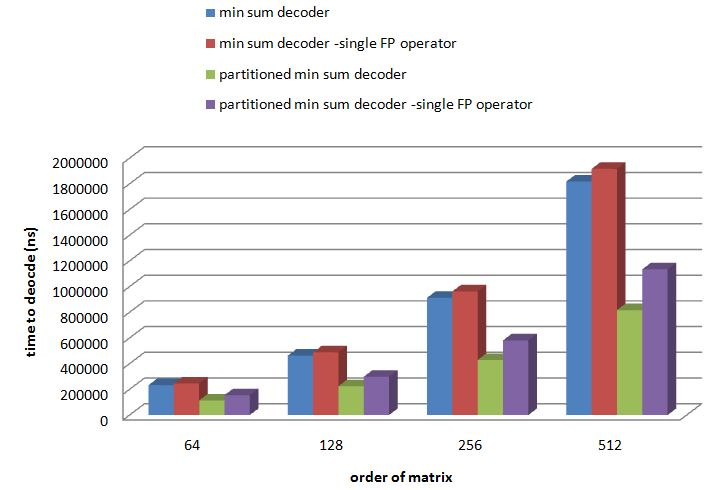
\includegraphics[height=6.5cm,width=11cm]{parallel_result1}
       \end{figure}
\end{frame}

\begin{frame}[t]
\vspace{-0.5cm} 
\frametitle{Results  }  
\begin{figure}
       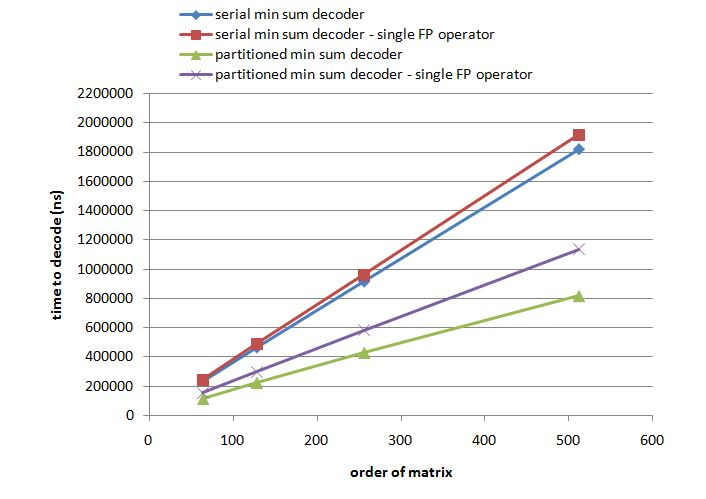
\includegraphics[height=6.5cm,width=11cm]{parallel_result2}
       \end{figure}
\end{frame}
%--------------------------------------------------------------
\begin{frame}[t]
\frametitle{Results} 
\begin{table}[]
\centering
\begin{tabular}{|p{1.3cm}|p{1.8cm}|p{1.8cm}|p{1.8cm}|p{1.8cm}|}
\hline
	& serial min sum decoder & serial min sum decoder \newline
	(single FP unit) & partitioned min sum decoder & partitioned min sum decoder(single FP unit) \\ \hline
FF & 18,076		&19,034		&49,854		&55,988 \\ \hline
LUT & 19,502  &20,621 &  51,929 & 60,296 \\ \hline
Memory LUT & 6 & 3 & 23 & 2 \\ \hline 
I/O & 128 & 128 & 128 & 128 \\ \hline
BRAM & 56 & 56 & 80 & 80 \\ \hline
BUFG  & 1 & 1 & 1 & 1 \\ \hline
\end{tabular}
\end{table}
\end{frame}
%-------------------------------------------------------------------
\section{Conclusions \& Future Work}
		\begin{frame} 
			\frametitle{Conclusion \& Future Work}
			
\begin{center}
\begin{tabular}{@{}cccc@{}}
\toprule
\textbf{Type of Matrix} & Gallager & Mackay Neal  &  Quasi-Cyclic  \\ 
\textbf{Performance Index} &  78\% & 86\% & 88\% \\ \bottomrule
\end{tabular}
\end{center}


\begin{itemize}
\setbeamertemplate{itemize item}[triangle]
\item The results show that a LDPC decoder can be parallelized with good efficiency.
\item The implemented 4-way partitioned decoder reduces the time required for decoding to half but uses 2.5$\times$ the harder required for single decoder.  
\item In future we can figure out a way to fold two engines on the top of other two engines to reduce hardware, instead of using four computational engines. 
\item The extension of the work can have different quantization levels of the floating point values and check for the trade off between accuracy of operation and error correcting threshold.
\end{itemize}
\end{frame}
%--------------------------------------------------------------------




%---------------------------end of document---------------------------	
\begin{frame}[plain]
\vspace{-20mm}
 			\begin{figure}
			
\includegraphics[height=10cm,width=11cm]{end}
			\end{figure}   
\end{frame}	



%----------------------------------------------------------------------

	\end{document}